\documentclass[12pt]{article}
\usepackage{verbatim}
\usepackage[dvips]{epsfig}
\usepackage[usenames]{color}
\usepackage{url}
\usepackage[colorlinks=true]{hyperref}

\begin{document}

\section*{GENESIS: Documentation}

{\bf Related Documentation:}
% start: userdocs-tag-replace-items related-do-nothing
% end: userdocs-tag-replace-items related-do-nothing

\section*{GENESIS Publication System}

The GENESIS Publication System supports the publication of new modeling projects and allows the manual incorporation of previous publications into a model lineage. The system is based on the traditional components of a paper based publication such as the Abstract, Introduction, Methods, Results, Discussion, Tables, Figures, and Appendices.

The submission, review, and publication of a completed modeling project is simplified by automated functionality which operates through the GENESIS GUI (\href{../gtube/gtube.tex}{\bf G-Tube}). 

The manual option is provided to enable integration of pre-existing publications into the publication system to enhance both data base searches  of model lineage and author attribution.

This document provides an overview of automated publication and outlines steps for the manual incorporation of pre-existing publications into the publication database of a given model. It relies on the file structure of project related publication in GENESIS. Manual incorporation can be done in either one of two ways:
\begin{enumerate}
\item {\bf Unitary Publication Database:} Provides a flat-file database that contains all files related to individual modeling projects in a single publication repository. The file structure of this repository is similar to that employed for user documentation.
\item {\bf Multiple Publication Database:} All files related to a given project are located in an unique project folder/directory in the publication repository to give a more hierarchical file system. It is this structure that is preferred for the GENESIS Publication System.
\end{enumerate}

\subsection*{The Publication Atom}

Publications are built from ``publication atoms''. These contain the smallest components of a project. For example, the publication Citation, an Abstract item, or sections in the Introduction, Methods, Results, Discussion,  or a Table or Figure of a traditional paper based publication. Automated publication defines publication atoms on the basis of the user and publication workflows. Both automated and manual publication are controlled by {\bf G-Tube}.

\subsection*{Automated publication}

Once completed, new GENESIS projects employ automated functionality to organize, check, and prepare projects for publication. This proceeds by allowing an investigator to use {\bf G-Tube} to flag the components of a project to be incorporated into a publication. Model related components of the submission are automatically checked prior to acceptance of a manuscript for review. The process generates a summary of project contents that is designed to simplify the review process.

\subsection*{Manual incorporation of pre-existing publications}

This option is made available to allow pre-existing publications to be incorporated into a publication data base to extend model lineage and enhance author attribution.

\subsubsection*{Manual generation of publication atoms}

The manual generation of publication atoms is based on extracting sections of a paper publication from the PDF file. For example, Figure\,\ref{fig:po-2} shows the first two pages of a paper publication. In this figure the red boxes identify text that will become the contents of the (1) model Citation, (2) first Abstract item, (3) first Figure, and (4) third Methods atom.

{\bf Note:} All other complete boxes in this figure also identify publication atoms. The Citation provides one atom, the Abstract can be divided into seven publication atoms, the Introduction provides one atom, and the Methods on the right hand page provide three complete publication atoms. The numbered atoms in this figure can be equated with with the yellow highlighted suggested filename Extension and the Atom tags given for this example in Figure\,\ref{fig:po-1} (See below.)

\begin{figure}[h]
  \centering
   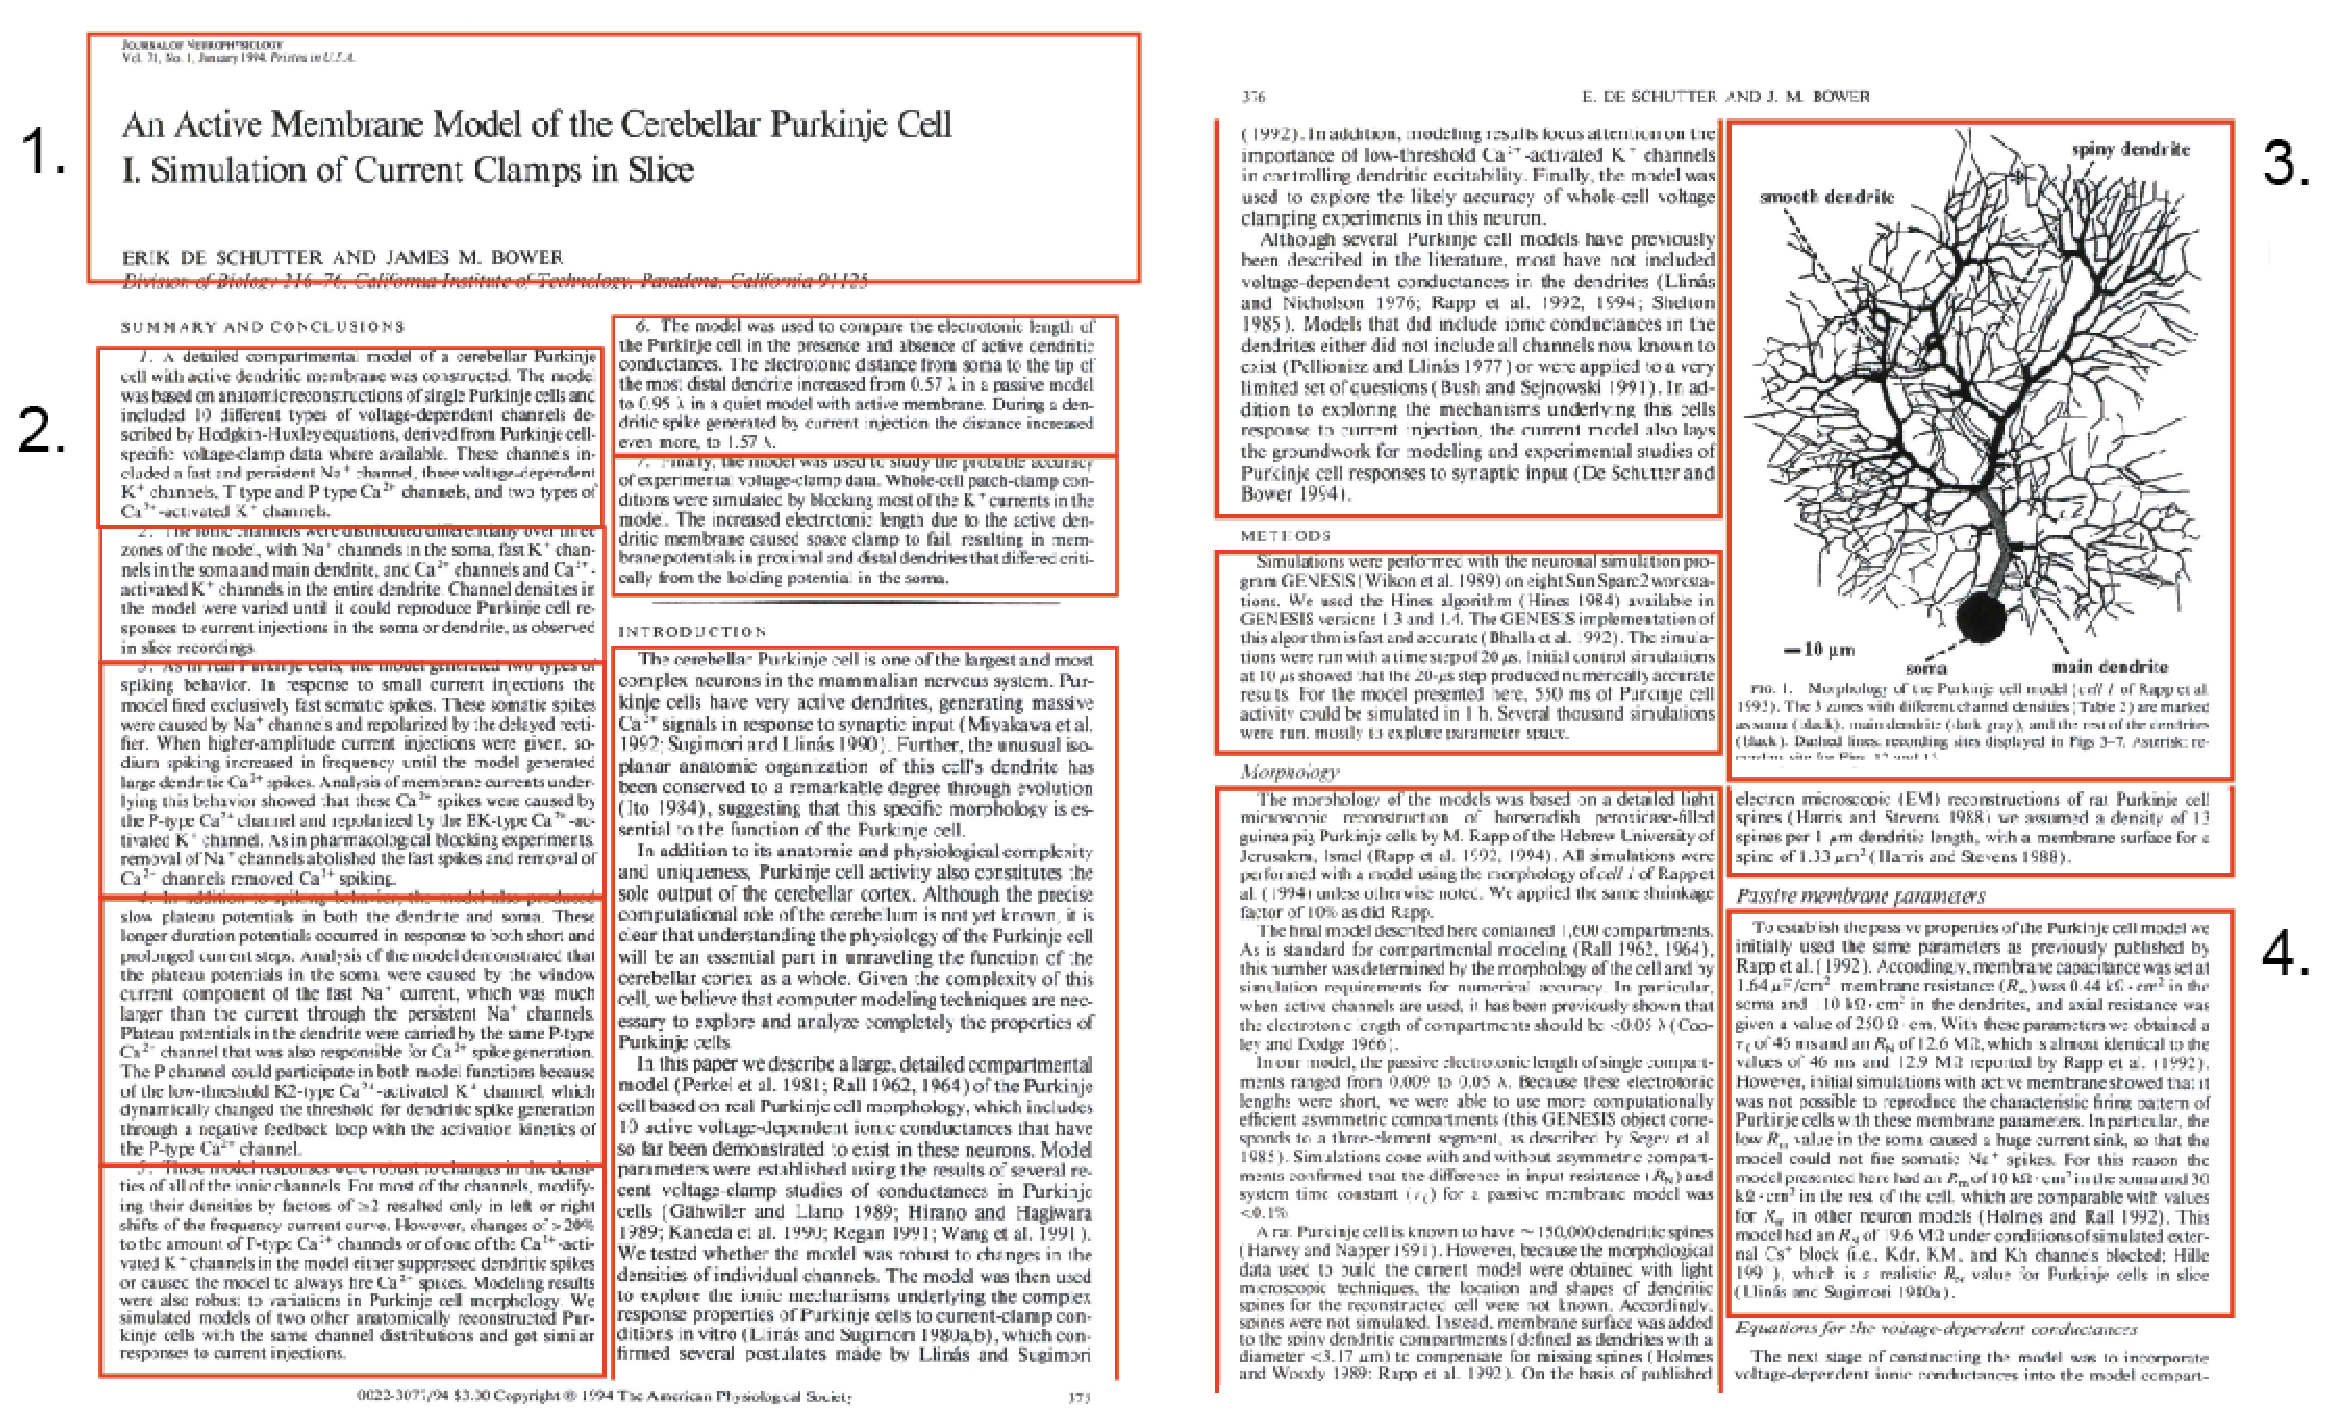
\includegraphics[scale=0.3]{figures/pub-manual-atoms-3.eps}
\caption{{\bf Identification of publication atoms in a previously published model.} This figure shows the first two pages of a paper publication. Each {\color{Red}{\bf red}} box identifies a ``publication atom''. The numbered boxes show examples of specific atoms--1. Citation, 2. First Abstract, 3. first Figure, and 4. third Methods atoms. See text for details.}
  \label{fig:po-2}
\end{figure}

\subsubsection*{Unitary publication database file naming conventions}

When all documents associated with individual publications or projects are located in a unitary publication database, e.g. 
\begin{verbatim}
   ~/neurospaces_project/publication/source/snapshots/0
\end{verbatim}   
each publication atom requires a unique file name. Figure\,\ref{fig:po-1} illustrates our approach in this case. The publication atoms of a given project are grouped by a `root'  identifier (e.g. {\tt pub-purkinje-deschutter-1}, {\color{Red}{\bf red}}) and each atom is identified by an `extension' (e.g. {\tt citation-1}, {\color{Green}{\bf green}}). This allows multiple publication atoms to exist within a single branch and to be grouped and uniquely identified by concatenation of the document class ({\tt pub}), cell type ({\tt purkinje}), specific model ({\tt deschutter-1}), and content ({\tt citation-1}), e.g {\tt pub-purkinje-deschutter-1-citation-1}.

\subsubsection*{Multiple publication database file naming conventions}

The unitary branch file naming convention outlined above can be greatly simplified by moving to a multiple publication database. In this case the publication repository contains multiple directory/folders which each contain all the publication atoms of a single publication. Advantages of this approach include: (i) simplification of automated publication atom naming, and (ii) elimination of the requirement for a root identifier as model identification can be based on the project citation.

\begin{figure}[h]
  \centering
   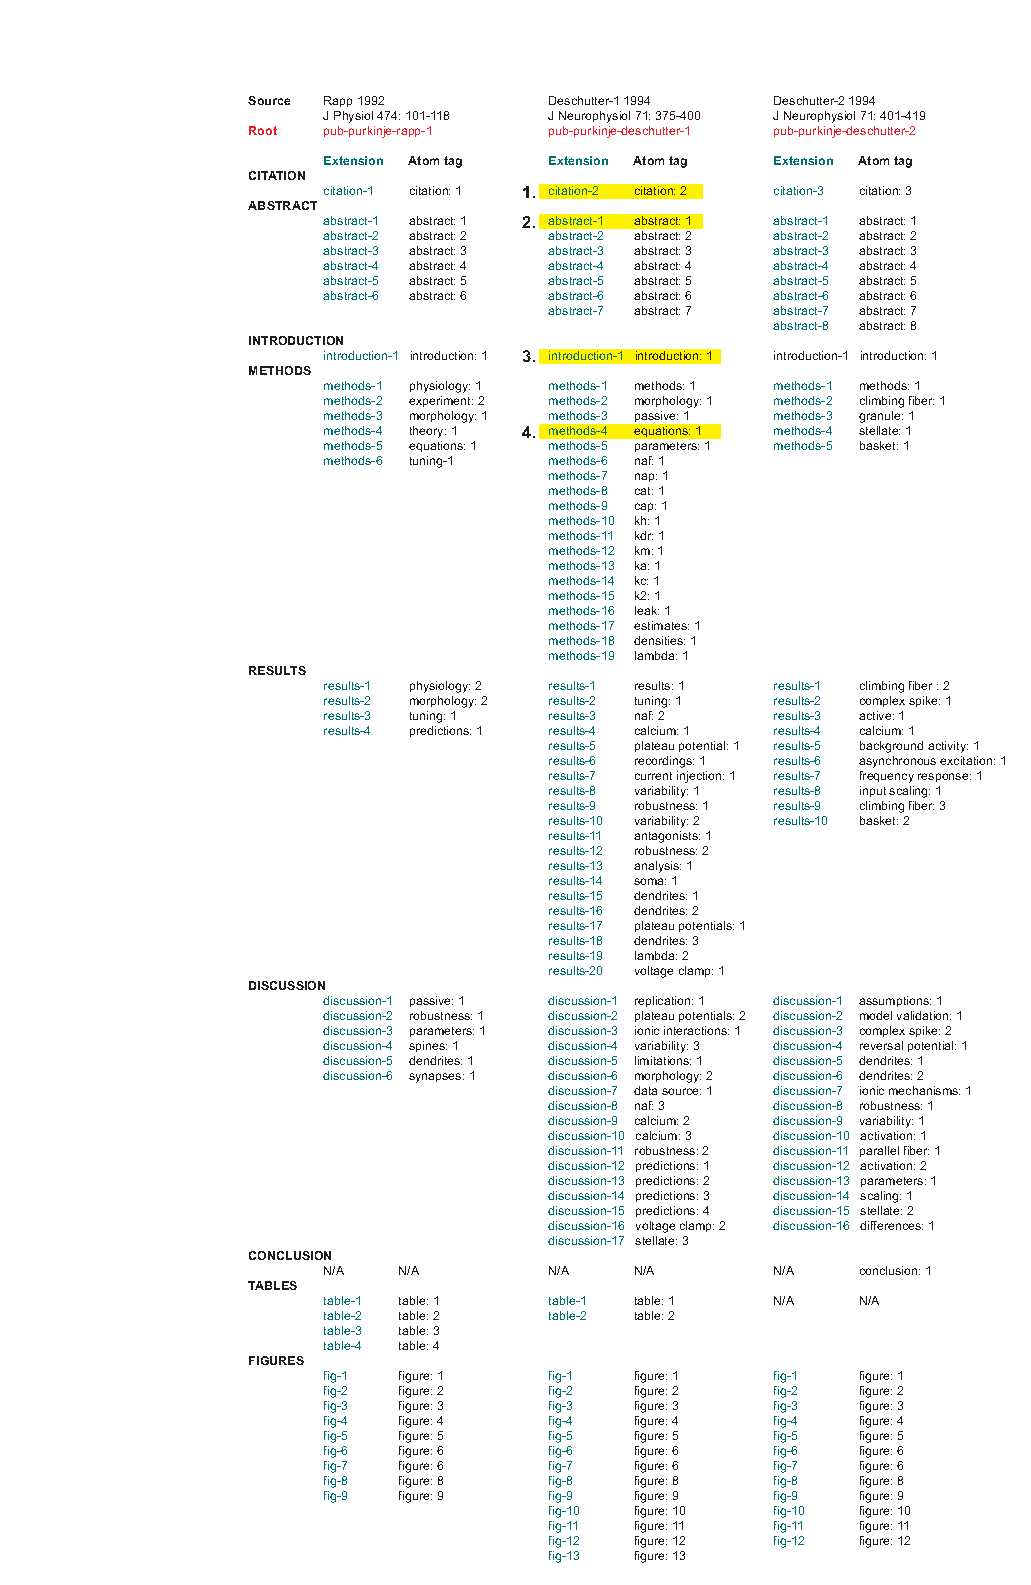
\includegraphics[scale=0.6]{figures/pub-overview.eps}
\caption{{\bf Naming conventions for manually generated publication atoms:} To identify each publication atom in a Unitary Publication Database, a `root' identifier ({\color{Red}{red}}) must be concatenated with a unique filename `extension' ({\color{Green}{green}}), whereas, in the Multiple Publication Database a root identifier is not required and the extension can be used as an unique filename within each project directory/folder. The {\bf Atom\,tag} refers to a tag incorporated into the {\it descriptoy.yml} file associated with each publication atom. It identifies the contents of the atom for database queries. See text for details.}
  \label{fig:po-1}
\end{figure}

\bibliographystyle{plain}
\bibliography{../tex/bib/g3-refs.bib}

\end{document}
